\documentclass[11pt]{article}
\usepackage[a4paper,margin=2.3cm]{geometry}
\usepackage[T1]{fontenc}
\usepackage{mathptmx}
\usepackage[scaled=0.9]{helvet}
\usepackage{courier}
\usepackage{microtype}
\usepackage{amsmath,amssymb}
\usepackage{bm}
\usepackage{graphicx}
\usepackage{booktabs}
\usepackage{tabularx}
\usepackage{array}
\usepackage[numbers,sort&compress]{natbib}
\usepackage{authblk}
\usepackage[font=small,labelfont=bf]{caption}
\usepackage{xcolor}
\usepackage{tikz}
\usetikzlibrary{positioning,arrows.meta,calc}
\usepackage[hidelinks]{hyperref}
\usepackage{lineno}
\linenumbers

\definecolor{rhy}{HTML}{2F6DB5}
\definecolor{mot}{HTML}{C8553D}
\definecolor{acc}{HTML}{2A9D8F}
\newcommand{\todo}[1]{\textcolor{mot}{[#1]}}
\newcolumntype{L}{>{\raggedright\arraybackslash}X}

\title{Rhythm without recruitment: a falsification-first audit of a connectome-constrained ventral nerve cord model as a controller for a simulated \textit{Drosophila} body}

\author[1]{Yupeng Ning\thanks{Correspondence: \href{mailto:ningyp@gmail.com}{ningyp@gmail.com}}}
\affil[1]{Beijing ZHYU Tech Corp, Beijing, China}
\date{Preprint --- \today}

\begin{document}
\maketitle

\begin{abstract}
\noindent
Connectome-constrained models of the \textit{Drosophila} ventral nerve cord (VNC) now reproduce rhythmic premotor activity under descending drive, inviting their use as body controllers. Through falsification tests, we asked whether the published rate model of the full male adult nerve cord (MANC; 23,532 neurons, 1,372,404 signed connections) can serve as such a controller. Across all 128 author-saved parameter sets under bilateral DNg100 drive, 51 produced sustained ${\sim}11$\,Hz rhythm in all six E1 premotor neurons, yet none showed co-modulated tibia flexor and extensor output in any leg: all 17 left-front tibia motor neurons were silent in every rhythmic set, 4.4--5.0 model units below threshold in five sets analysed in detail despite incoming weights identical to those of a recruiting set. The ensemble split into two regimes ($\leq$38 versus $\geq$289 of 732 motor neurons active), and antagonistic tibia output occurred only in the hyperactive one (9 of 10 versus 0 of 118 sets; Fisher's exact $p=5\times10^{-13}$), where E1 rhythm was absent or confined to at most two hemisegments. Tonic current into a flexor premotor neuron recruited only unmodulated flexor output, closing a sensory loop with a physical body left all front- and middle-leg tibia pools subthreshold, and replaying the saved motor output into two six-legged bodies produced no walking (0/256 runs). We also document four pitfalls producing false positives or negatives: a walker that passed a locomotion gate behaved bit-identically when its network input was replaced by a replayed phase signal; fixed-step Euler integration changed rhythm classification in 6 of 32 full-network sets; a gait gate accepted a foot-dragging controller; and a peak-based detector undercounted ${\sim}11$\,Hz rhythm tenfold (5 versus 51 sets). We propose these controls as minimal acceptance tests for connectome-to-body claims and identify motor-neuron recruitment, not rhythm generation, as the bottleneck in this model class.
\end{abstract}

\section{Introduction}

Complete synapse-resolution connectomes of the adult \textit{Drosophila} central nervous system have made it possible to build network models whose architecture is fixed by anatomy rather than fitted to behaviour \citep{takemura2024manc,marin2024manc,cheong2024premotor,shiu2024brain}. For locomotion, Pugliese et al.\ simulated rate models of the male adult nerve cord (MANC) and showed that sustained input to the descending neuron DNg100 elicits rhythmic activity in leg premotor circuits, from which they isolated a small excitatory--inhibitory core (E1/E2/I1) able to generate the rhythm \citep{pugliese2026}. Experimental work has since described per-leg rhythm modules, descending co-activation (DNg100 with DNg97), and sensory shaping of the step cycle \citep{sapkal2026}. In parallel, anatomically detailed body models and physics engines make it technically straightforward to attach such a network to a simulated fly \citep{todorov2012mujoco,wangchen2024nmf,vaxenburg2025flybody,ozdil2025flymimic}.

The step from ``the network oscillates'' to ``the network walks the body'' is, however, easy to overclaim. A recent cautionary study paired a nematode connectome with a fly body and trained controller and still obtained realistic-looking fly walking \citep{brunton2026sphinx}: behavioural realism alone does not show that the connectome is doing the work. At least four distinct properties are involved: (i) the network dynamics must be numerically valid; (ii) premotor rhythm must be present; (iii) motor neurons (MNs) must be recruited in an antagonistic, leg-specific pattern; and (iv) that output, through muscles and ground contact, must move a body in a way that depends causally on the network's online state.

Here we report a systematic attempt to satisfy all four with the published MANC rate model, organised as falsification tests with pre-specified or explicitly flagged post-hoc criteria (Table~\ref{tab:overview}). The attempt did not produce connectome-driven walking. We report the resulting negative result, which localises the failure at level (iii), together with four controls that each caught a false positive or a false negative during the project and that we believe generalise to other connectome-to-body efforts (Fig.~\ref{fig:ladder}).

\begin{figure}[t]
\centering
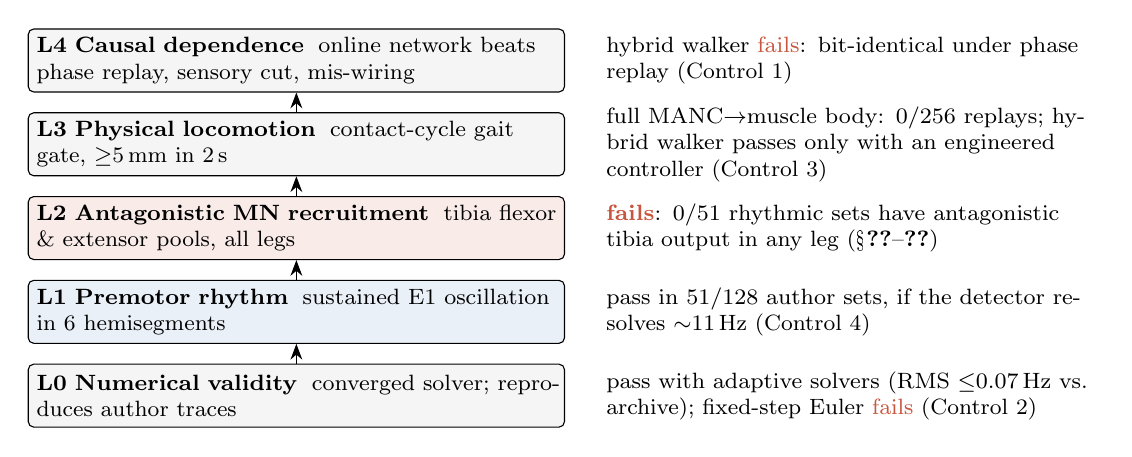
\begin{tikzpicture}[
  node distance=2.5mm,
  lvl/.style={draw, rounded corners=2pt, text width=6.6cm, minimum height=8mm, align=left, font=\footnotesize, inner sep=3pt},
  stat/.style={font=\footnotesize, align=left, anchor=west, text width=6.2cm}]
\node[lvl, fill=gray!8] (l0) {\textbf{L0 Numerical validity}\; converged solver; reproduces author traces};
\node[lvl, fill=rhy!10, above=of l0] (l1) {\textbf{L1 Premotor rhythm}\; sustained E1 oscillation in 6 hemisegments};
\node[lvl, fill=mot!12, above=of l1] (l2) {\textbf{L2 Antagonistic MN recruitment}\; tibia flexor \& extensor pools, all legs};
\node[lvl, fill=gray!8, above=of l2] (l3) {\textbf{L3 Physical locomotion}\; contact-cycle gait gate, $\geq$5\,mm in 2\,s};
\node[lvl, fill=gray!8, above=of l3] (l4) {\textbf{L4 Causal dependence}\; online network beats phase replay, sensory cut, mis-wiring};
\foreach \a/\b in {l0/l1,l1/l2,l2/l3,l3/l4} \draw[-{Stealth[length=2mm]}] (\a) -- (\b);
\node[stat, right=4mm of l0] {pass with adaptive solvers (RMS $\leq$0.07\,Hz vs.\ archive); fixed-step Euler \textcolor{mot}{fails} (Control 2)};
\node[stat, right=4mm of l1] {pass in 51/128 author sets, if the detector resolves ${\sim}11$\,Hz (Control 4)};
\node[stat, right=4mm of l2] {\textcolor{mot}{\textbf{fails}}: 0/51 rhythmic sets have antagonistic tibia output in any leg (\S\ref{sec:r1}--\ref{sec:r3})};
\node[stat, right=4mm of l3] {full MANC$\rightarrow$muscle body: 0/256 replays; hybrid walker passes only with an engineered controller (Control 3)};
\node[stat, right=4mm of l4] {hybrid walker \textcolor{mot}{fails}: bit-identical under phase replay (Control 1)};
\end{tikzpicture}
\caption{\textbf{Validation ladder used in this study.} Each level is necessary for a claim that a connectome-constrained network drives locomotion; passing a higher level does not certify a lower one. Right: status of the MANC rate model and of a hybrid walker (network phase driving a trained joint-space controller) in this study.}
\label{fig:ladder}
\end{figure}

\section{Methods}

\subsection{Network model and data provenance}
We used the MANC rate model, parameters and code of Pugliese et al.\ \citep{pugliese2026} (MIT-licensed code, commit \texttt{10e7661}; CC-BY-4.0 data, Zenodo record 22260924). The full network comprises 23,532 neurons and 1,372,404 nonzero directed signed connections from the 2025-10-06 MANC export that matches the archived parameters; we did not substitute newer connectome releases because node indices differ. Neuron rates follow the authors' first-order equation, $\tau_i\,\dot r_i=-r_i+\max\{0,\;c_i\tanh[(a_i/c_i)(I_i^{\text{ext}}+\sum_j w_{ij}r_j-\theta_i)]\}$, with per-neuron time constants $\tau_i$, gains $a_i$, rate caps $c_i$ and thresholds $\theta_i$, and signed synaptic weights scaled by the authors' excitatory and inhibitory multipliers (both 0.03 in the runs analysed). All currents and margins below are in the model's internal units and are not calibrated to physiological currents.

We obtained the authors' archived sparse rate tensors for four full-MANC runs (\texttt{30662613}, \texttt{33195857}, \texttt{33195876}, \texttt{33195882}), each containing 32 parameter sets (128 in total; indexed below as ``set'' by the global row of the authors' Figure~4), 2\,s at 1\,ms resolution, with bilateral DNg100 input of 380 units from 0.02 to 1.999\,s and network pruning disabled. Only the required archive members were extracted by HTTP byte range; sizes, CRC32 and SHA-256 were recorded. As a reproduction check, the number of active MNs per set recomputed from the archived tensors matched the authors' Figure~4 in 128/128 sets. When we re-integrated the network ourselves, we used an independent SciPy RK45 (Dormand--Prince 5(4)) integrator \citep{dormand1980} with $\mathrm{rtol}=2\times10^{-6}$, $\mathrm{atol}=5\times10^{-9}$ and maximum step 1\,ms, and, where noted, the authors' own Diffrax Dopri5 solver with identical tolerances \citep{kidger2021thesis}. The RK45 re-integration reproduced the archived rates of the six E1 neurons and 732 MNs with RMS error $2.8\times10^{-4}$\,Hz for set 45, and reproduced the E1 traces with RMS errors of 0.066 and 0.023\,Hz for sets 122 and 126 (run \texttt{33195882}, rows 26 and 30; Control~2).

\subsection{Neural read-outs and statistics}
Neurons were identified from the matching MANC annotation: six E1 neurons (type IN17A001), 732 MNs, and, per leg, the ``tibia flex'' and ``tibia extend'' motor modules (86 cells in total, 74 flexor and 12 extensor MNs; 15 flexor and 2 extensor MNs in the left front leg). All read-outs use 0.5--2.0\,s.
\emph{Sustained E1 rhythm (primary, spectral).} From the 1\,ms trace, peak-to-peak amplitude $\geq$2\,Hz; after linear detrending and a Hann window, the dominant frequency in 2--50\,Hz must carry $\geq$30\% of the 1--100\,Hz power within $\pm\max(1.5\,\mathrm{Hz}, 15\%)$ of the peak; and the final-third amplitude must be at least half of the first-third amplitude (for re-integrations saved only at 10\,ms resolution, the same criterion was applied to the 10\,ms samples).
\emph{Sustained E1 rhythm (secondary, peak-based).} The criterion inherited from the project's original pipeline: on 10\,ms samples, $\geq$5 peaks (prominence $\geq\max(0.5, 0.1\times\text{amplitude})$, minimum spacing 10 samples), coefficient of variation of inter-peak intervals $\leq$0.2, same amplitude and sustain conditions. Its 100\,ms minimum spacing cannot follow oscillations faster than 10\,Hz (Control~4).
\emph{Antagonistic tibia modulation} (per leg): both the flexor and the extensor pool must contain $\geq$1 neuron exceeding 1\,Hz, and each pool-mean rate must vary by $\geq$0.5\,Hz. This is deliberately permissive---it does not require alternation---so failing it is informative.
\emph{MN activity}: the number of the 732 MNs exceeding 1\,Hz.
\emph{Threshold margin}: for a MN $i$, $m_i(t)=I_i^{\text{ext}}(t)+\sum_j w_{ij}\,r_j(t)-\theta_i$, the argument of the nonlinearity; a neuron with $m_i<0$ throughout cannot fire in this model.
\emph{Statistics}: associations across parameter sets were tested with two-sided Fisher's exact tests, treating the 128 sets as independent draws; robustness was assessed over three E1 detectors and three tibia thresholds (Table~\ref{tab:robust}). The spectral detector and the two-regime split (a gap in MN activity between 38 and 289 active MNs) were defined after inspecting the data and should be regarded as exploratory.

\subsection{Bodies and physical gates}
All bodies were simulated in MuJoCo \citep{todorov2012mujoco}. (a) A free six-legged body with 78 Hill-type muscles, obtained by transferring the published left-front-leg musculoskeletal template \citep{ozdil2025flymimic} to all legs along bone axes; this transfer is an uncalibrated engineering assumption (the released model contains active muscles for one leg only). MN rates were pooled per muscle family through an uncalibrated rate-to-excitation mapping. (b) A free body with 18 motor-family joint torques. (c) The \texttt{fruitfly\_v1} body with 56 direct joint actuators from a recent whole-body 3D kinematics study \citep{ispizua2026kinematics}, driven by a trained joint-space controller conditioned on a phase variable (the ``hybrid walker'').
\emph{Gate for MN-output replays} (bodies a and b): $\geq$5\,mm forward displacement in 2\,s, upright posture and body clear of the ground in $\geq$99\% of samples, $\geq$2 complete steps per leg, median stance slip $<$2\,mm\,s$^{-1}$, and foot-only support in $\geq$99\% of samples.
\emph{Original gate for the hybrid walker} (body c): $\geq$5\,mm in 2\,s, body--ground contact $\leq$5\% of frames and $\geq$2 toe-height cycles per leg.
\emph{Contact-cycle gate} (body c): the original gate plus, per leg, $\geq$2 complete stance$\rightarrow$swing$\rightarrow$stance cycles with each phase lasting $\geq$7 frames at 800\,Hz (8.75\,ms), foot-only support in $\geq$99\% of frames, and median planted-foot slip $\leq$1.25$\times$ that of a real-fly reference bout replayed on the same body (5.10\,mm\,s$^{-1}$; limit 6.37\,mm\,s$^{-1}$). The real-fly data comprise 53 flies, 2,213 running bouts and 653,919 frames at 800\,Hz \citep{ispizua2026kinematics}. The contact-cycle thresholds were set \emph{after} the frozen-network result was seen (Control~3) and should be treated as exploratory until re-validated on held-out bouts.

\subsection{Provenance of analyses}
The simulations and analyses of the original project were executed by an autonomous large-language-model coding agent running on the author's workstation, with an independent re-computation script for each reported result. Its outputs were subsequently audited by the author with the assistance of a second AI model, which re-derived every number reported here from the saved result files, re-analysed the archived trajectories with the spectral detector, and ran the full-network integrator comparison in Control~2. Figures and tables were regenerated directly from the saved files by scripts that also write every plotted value to a machine-readable file (Data and code availability).

\begin{table}[t]
\centering
\caption{\textbf{Overview of experiments.} Set numbers refer to global rows of the authors' Figure~4. ``Author archive'' denotes rates saved by the model's authors with their adaptive solver.}
\label{tab:overview}
\footnotesize
\begin{tabularx}{\linewidth}{@{}>{\raggedright\arraybackslash}p{2.5cm}L>{\raggedright\arraybackslash}p{2.3cm}>{\raggedright\arraybackslash}p{2.2cm}L@{}}
\toprule
Experiment & Network and input & Integration & Body & Outcome \\
\midrule
Ensemble screen (\S\ref{sec:r1}) & Full MANC, 128 author sets, bilateral DNg100 & Author archive & --- & Six-leg E1 rhythm in 51 sets; antagonistic tibia output in any leg in 9 sets; overlap 0 \\
MN-output replay (\S\ref{sec:r1}) & Saved MN rates of all 128 sets & --- & 78-muscle; 18-torque & 0/256 pass; best 0.648\,mm \\
Threshold margins (\S\ref{sec:r2}) & 7 sets, archived rates and same-run weights & Author archive & --- & Rhythmic sets: 17 LF tibia MNs 4.4--5.0 below threshold \\
Premotor current (\S\ref{sec:r3}) & Set 45; IN21A004 $+80$/$+160$, IN04B031 $+60$ & RK45 & --- & E1 rhythm kept (6/6); 2--4/15 LF flexors tonic; extensors 0/2 \\
Sensory loop (\S\ref{sec:r3}) & Set 117; DNg100 + DNg75; FeCO and load feedback & RK45 per 10\,ms & 78-muscle & T1--T2 tibia pools subthreshold; $\leq$0.005\,mm \\
Control 1 & Full MANC online vs.\ replayed phase & Euler 1\,ms & 56-actuator, trained controller & Bit-identical from 4/4 starts \\
Control 2 & T1 sub-network (1,856 settings); full MANC, 32 sets & Euler 1--0.1\,ms vs.\ RK45, Dopri5 & --- & Euler-only candidates vanish; 6/32 sets misclassified at 1\,ms \\
Control 3 & Four-cell E1/E2/I1 core, intact vs.\ frozen & Core model & 56-actuator, trained controller & Frozen passes kinematic gate, fails contact gate \\
Control 4 & 128 author sets & Author archive & --- & Peak detector 5/128 vs.\ spectral 51/128 rhythmic sets \\
\bottomrule
\end{tabularx}
\end{table}

\section{Results}

\subsection{Six-leg rhythm and antagonistic tibia output occupy disjoint regimes}
\label{sec:r1}
We first screened the 128 author-saved trajectories without any re-integration. Sustained E1 rhythm in all six hemisegments occurred in 51/128 sets, at a median frequency of 11.3\,Hz (interquartile range 11.0--12.0\,Hz across sets). None of these 51 sets showed antagonistic tibia modulation in any leg (Fig.~\ref{fig:screen}A,B). Antagonistic modulation in all six legs occurred in only two sets (2 and 117), and in at least one leg in nine sets, which showed sustained E1 rhythm in at most two hemisegments. The joint target of six-leg rhythm with six-leg antagonism was therefore empty. Because six-leg recruitment is rare, an empty intersection alone is weak evidence (with 51 rhythmic and 2 recruiting sets it would occur with probability 0.36 even if the two properties were independent); the graded pattern is more informative: rhythm and recruitment were strongly anti-associated across sets (sets with any E1 rhythm versus sets with any recruiting leg, Fisher's exact $p=6.4\times10^{-6}$), and this held for every combination of three E1 detectors and three tibia thresholds (Table~\ref{tab:robust}).

The ensemble also split sharply by overall MN activity (Fig.~\ref{fig:screen}C). In 118 sets at most 38 of the 732 MNs exceeded 1\,Hz; in the other 10 sets, 289--439 did, with no set in between. All 51 rhythmic sets lay in the low-activity regime, where they recruited 13--38 MNs (median 20): mostly femur/trochanter (36\% of active MNs) and coxa pools (23\%) and MNs without a leg motor module (26\%), plus about two tibia extensor MNs per set (10\%); tibia flexor MNs were active in only 2 of the 3,774 flexor--set combinations, and the 17 left-front tibia MNs never fired (maximum rate 0\,Hz in all 51 sets). All nine sets with a recruiting leg lay in the hyperactive regime (9 of 10 hyperactive sets versus 0 of 118 low-activity sets; $p=5.2\times10^{-13}$). This extends the authors' observation that DNg100 drive recruits only a small number of leg MNs \citep{pugliese2026}: in this parameter ensemble, the low-activity regime that supports six-leg rhythm recruits femoral and coxal pools and tibia extensors but not tibia flexors, and the only route to tibia flexor--extensor co-activity is a hyperactive regime in which rhythm collapses.

\begin{table}[t]
\centering
\caption{\textbf{Robustness of the rhythm--recruitment dissociation} across E1 detectors and tibia thresholds (active cell $>$\,$x$\,Hz; pool-mean modulation $\geq$\,$y$\,Hz). Entries: sets with six-leg E1 rhythm / sets with six-leg antagonistic tibia output / joint / six-leg-rhythmic sets with any recruiting leg; Fisher's exact $p$ for any E1 rhythm versus any recruiting leg. Default settings in bold.}
\label{tab:robust}
\footnotesize
\begin{tabular}{@{}lccc@{}}
\toprule
E1 detector & lenient (0.1\,Hz; 0.1\,Hz) & \textbf{default (1\,Hz; 0.5\,Hz)} & strict (5\,Hz; 2\,Hz) \\
\midrule
Peak-based (inherited) & 5/2/0/1; $p=5.7\times10^{-9}$ & 5/2/0/0; $p=1.3\times10^{-9}$ & 5/1/0/0; $p=2.3\times10^{-6}$ \\
\textbf{Spectral, concentration $\geq$0.3} & 51/2/0/2; $p=1.8\times10^{-5}$ & \textbf{51/2/0/0}; $\bm{p=6.4\times10^{-6}}$ & 51/1/0/0; $p=4.2\times10^{-4}$ \\
Spectral, concentration $\geq$0.5 & 36/2/0/2; $p=1.8\times10^{-6}$ & 36/2/0/0; $p=2.8\times10^{-7}$ & 36/1/0/0; $p=1.7\times10^{-5}$ \\
\bottomrule
\end{tabular}
\end{table}

\begin{figure}[p]
\centering
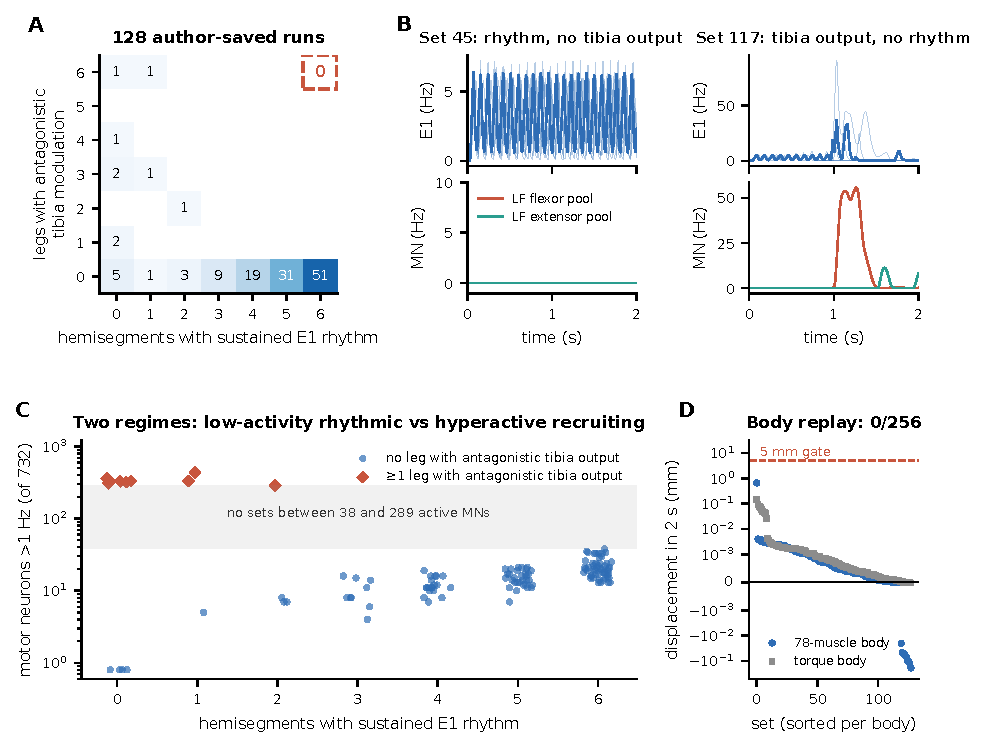
\includegraphics[width=\linewidth]{figures/fig2_rhythm_vs_recruitment.pdf}
\caption{\textbf{Rhythm and recruitment occupy disjoint regimes across the 128 author-saved full-MANC runs.} \textbf{A}, Number of hemisegments with sustained E1 rhythm (spectral detector) versus number of legs with co-modulated tibia flexor and extensor pools. The joint target (6,6; dashed) is empty; all 51 fully rhythmic sets have zero recruiting legs. \textbf{B}, Archived rates for a rhythmic set (45) and a recruiting set (117): six E1 neurons (thin; left-front E1 bold) and the left-front tibia flexor and extensor pool means. \textbf{C}, MN activity versus E1 rhythm; sets with a recruiting leg (diamonds) all lie in a hyperactive regime separated from the rest by a gap (shaded; sets with no active MN drawn at 0.8). \textbf{D}, Forward displacement in 2\,s when each set's saved MN output drives the 78-muscle Hill body or the 18-family torque body (each sorted independently; symmetric-log axis). No run approached the 5\,mm gate (best 0.648 and 0.142\,mm, both set 117); 15 and 5 runs moved backwards (down to $-0.18$\,mm).}
\label{fig:screen}
\end{figure}

To test whether a body could nonetheless extract locomotion from these outputs, we replayed each set's saved MN rates, without any added phase or gait signal, into the two free six-legged bodies. None of the 256 runs met the replay gate or reached 5\,mm (Fig.~\ref{fig:screen}D). The best run (set 117, Hill body) moved 0.648\,mm with per-leg step counts of $[0,3,0,0,2,0]$; medians were $5.4\times10^{-4}$ and $7.3\times10^{-4}$\,mm. Part of this failure lies at the interface: in set 117, 189 annotated leg MNs were active after 0.5\,s, of which 154 mapped to a muscle of the Hill body and 35 had no muscle outlet. Because both body models lack measured six-leg muscle parameters, this replay cannot on its own exclude that a correctly calibrated body would walk; the neural screen in Fig.~\ref{fig:screen}A--C does not depend on any body.

\subsection{In rhythmic regimes, tibia motor neurons sit just below threshold}
\label{sec:r2}
We next asked why. For seven representative sets---the five that are rhythmic under both E1 detectors and the two six-leg recruiting sets---we reconstructed, from the archived rates and the same-run weights, the threshold margin of all 17 left-front tibia MNs. In the five rhythmic sets every one of these neurons remained below threshold at every 10\,ms sample of the 0.5--2.0\,s window, with the largest margin across the 17 cells between $-4.37$ and $-5.04$ (Fig.~\ref{fig:mech}A). In the two recruiting sets the margins were $+1{,}683$ and $+2{,}196$. The comparison between set 45 (rhythmic) and set 117 (recruiting) is instructive: the incoming weight columns and masks of the 17 MNs were bit-identical, and mean thresholds differed only modestly (20.75 vs.\ 19.33), whereas mean excitatory and inhibitory input differed 30--50-fold (3.29 and $-8.31$ vs.\ 155.24 and $-256.54$). The difference is therefore carried by upstream network state rather than by MN parameters. A retrospective decomposition of the additional net drive to the flexor MN 12134 in set 117 relative to set 45 ($+326.9$) identified the two largest positive contributors as IN21A004 (body ID 12650; $+219.0$) and IN03A004 (10827; $+157.6$), both silent in set 45.

\begin{figure}[t]
\centering
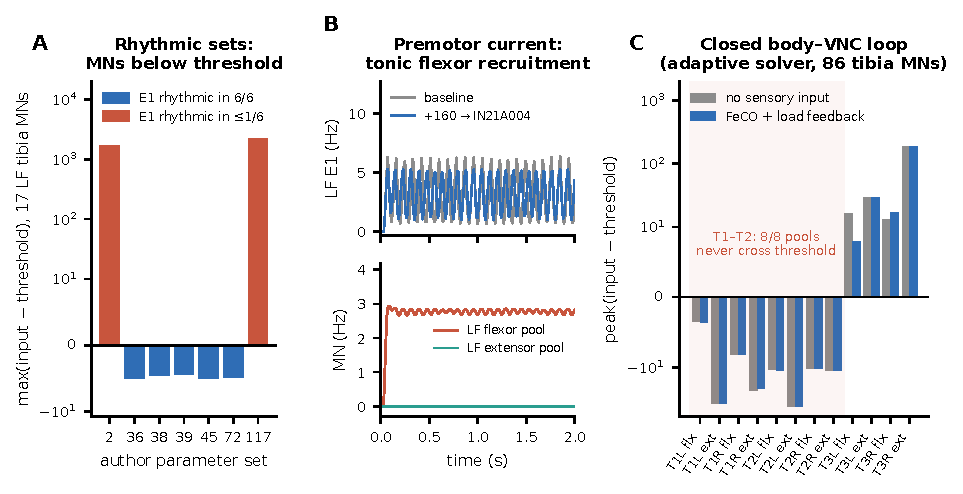
\includegraphics[width=\linewidth]{figures/fig3_subthreshold_mechanism.pdf}
\caption{\textbf{The failure is localised at motor-neuron recruitment.} \textbf{A}, Largest threshold margin among the 17 left-front tibia MNs, 0.5--2.0\,s, for seven author sets (symmetric-log axis). Rhythmic sets (blue) never cross threshold; recruiting sets (red) lack E1 rhythm. \textbf{B}, Constant current ($+160$) into the flexor premotor neuron IN21A004 (12650) in the full network (set 45, RK45): the left-front E1 keeps oscillating (6/6 hemisegments rhythmic), four of 15 left-front flexor MNs are recruited but their pool rate is nearly constant, and the extensor pool stays at zero. \textbf{C}, Closed loop with the Hill body (set 117 parameters with bilateral DNg100 and DNg75 drive; RK45 within 10\,ms exchange intervals): peak margin of all 12 tibia pools with and without FeCO velocity and load feedback. All eight front- and middle-leg pools stay below threshold.}
\label{fig:mech}
\end{figure}

\subsection{Tonic premotor drive recruits flexors without antagonism; sensory feedback does not rescue recruitment}
\label{sec:r3}
If the bottleneck lies upstream, driving the identified premotor neurons should recruit MNs. Using the RK45 re-integration of set 45 (which reproduces the authors' traces, Methods), we added constant current to IN21A004 (Fig.~\ref{fig:mech}B). At $+80$ units the neuron fired at 10.9\,Hz (mean after 0.5\,s) and its target flexor MN 12134 at 4.4\,Hz, recruiting 2 of 15 left-front flexor MNs; at $+160$ they fired at 25.4 and 20.2\,Hz and 4 of 15 flexors were recruited. E1 rhythm persisted in all six hemisegments in every condition, but the flexor pool-mean rate varied by only 0.26 and 0.19\,Hz, below the 0.5\,Hz modulation criterion, and the two left-front extensor MNs stayed silent; adding $+60$ to the extensor premotor neuron IN04B031 (17678; 12.9\,Hz) did not recruit the extensor MN 12704. Tonic activation of an identified premotor pathway therefore lifts flexor MNs above threshold without phase-locking them to the rhythm or engaging their antagonists.

Because sensory feedback shapes the step cycle in flies \citep{sapkal2026,dallmann2025presynaptic}, we closed the loop through the body: joint-velocity (FeCO; SNpp39/41) and load (SNpp53) signals computed from the Hill body were injected into the corresponding annotated MANC sensory neurons every 10\,ms, with the network integrated adaptively in between. Feedback measurably changed network activity (mean absolute change 0.067\,Hz across the 738 recorded neurons), and cutting all output synapses of the stimulated sensory neurons returned the network to the no-feedback trajectory to within $8.7\times10^{-5}$\,Hz on average. Nevertheless, the eight front- and middle-leg tibia pools remained below threshold (Fig.~\ref{fig:mech}C), and the body moved only 0.0017--0.0046\,mm in 2\,s across four conditions. In earlier fixed-step simulations, injecting all annotated leg sensory classes at once destabilised the network; in a class-wise screen, angle-encoding SNpp50/51 input was destabilising whereas SNpp53 and SNpp39/41 input was not, but the latter had no measurable functional benefit under sensory deafferentation, left--right mis-wiring or a single-leg joint perturbation. Because transduction gains are unmeasured and those screens used fixed-step integration, we treat all sensory results as exploratory.

\subsection{Four controls that each caught a false positive or negative}
\label{sec:controls}

\paragraph{Control 1: online network versus replayed phase.}
In a hybrid configuration, the full 23,532-neuron MANC (run \texttt{33195882}, row 13, integrated with 1\,ms Euler steps) ran online alongside the 56-actuator body; a single phase variable read from left-front E1/E2/I1 conditioned a trained joint-space controller. This system passed the original locomotion gate from 4/4 initial states (19.4--33.3\,mm in 2\,s). We then deleted the network at runtime and fed the controller only the phase trajectory recorded from a previous run. Body state and all 56 actuator commands were bit-identical to the online run in all 1,601 frames for all four initial states (Fig.~\ref{fig:controls}A). The network was thus acting as an open-loop clock with no online, body-dependent role; its 732 MNs averaged 0.029\,Hz. This conclusion does not depend on the accuracy of the fixed-step integration. It is the specific failure mode highlighted by the ``digital sphinx'' study \citep{brunton2026sphinx}, and it is cheap to detect: replacing the network by its own recorded output should be a mandatory control.

\paragraph{Control 2: integrator convergence.}
In the 4,604-neuron prothoracic (T1) sub-network of the authors' DNg100 model, a screen of 116 published synaptic-multiplier settings $\times$ 16 parameter rows (1,856 simulations) with fixed-step Euler at 1\,ms found one candidate (multiplier setting 90, row 10) with left-front E1 rhythm and anti-correlated tibia flexor/extensor pools, and a second (row 78) among the remaining 112 rows. Both disappeared under Euler at 0.5, 0.25 and 0.125\,ms, under independent RK45, and under the authors' own Dopri5 solver (Fig.~\ref{fig:controls}B): for row 10, the 1\,ms Euler oscillation of E1 is a discretisation artefact, and the flexor--extensor correlation changed sign from $-0.59$ to $+0.19$. Small-step Euler and the adaptive solvers agree qualitatively (no oscillation) but not in steady-state level, underlining that step-size reduction alone is not a convergence proof. The full network showed the same sensitivity. Integrating the 32 sets of run \texttt{33195882} with 1\,ms Euler steps changed the number of rhythmic E1 hemisegments relative to the authors' archived adaptive solution in 6 of 32 sets. For sets 122 and 126 (rows 26 and 30), the archive and our RK45 re-integration agreed (E1 RMS differences 0.066 and 0.023\,Hz; 6/6 rhythmic hemisegments), whereas Euler at 1 and 0.5\,ms produced large-amplitude spurious dynamics (0/6 hemisegments classified as rhythmic; RMS deviations of 22.6 and 12.8\,Hz at 1\,ms) and set 122 remained misclassified even at 0.1\,ms (2/6; RMS deviation 12.4\,Hz; Fig.~\ref{fig:controls}C). We therefore required every neural candidate to be confirmed with an adaptive solver before any body experiment.

\paragraph{Control 3: kinematic versus contact-cycle gait gate.}
With the hybrid walker driven by the four-cell E1/E2/I1 core, the intact network produced 38.2\,mm of forward travel from the standard start, and freezing the network state still produced 18.5\,mm. Both passed the original gate, because the frozen condition produced many toe-height peaks (17--57 per leg). Counting complete stance--swing--stance contact cycles instead revealed that the frozen controller made zero such cycles in three legs (LF, RF, LM), with a median planted-foot slip of 11.9\,mm\,s$^{-1}$ versus 4.4\,mm\,s$^{-1}$ for the intact network and 5.1\,mm\,s$^{-1}$ for real flies (Fig.~\ref{fig:controls}D): it was dragging rather than stepping. Under the contact-cycle gate the intact core passed from 2/3 held-out initial states and the frozen core from 0/3; silencing E1 or E2 also failed (3.4 and 4.4\,mm). These results show a functional dependence of the hybrid controller on the core rhythm, but, per Control 1, not connectome-driven walking.

\paragraph{Control 4: detector resolution.}
The rhythm detector inherited from the project's original pipeline required peaks at least 100\,ms apart on 10\,ms samples and a coefficient of variation of inter-peak intervals $\leq$0.2. Because E1 oscillates at ${\sim}11$\,Hz (period ${\sim}90$\,ms), this spacing forces the detector to skip cycles irregularly (Fig.~\ref{fig:controls}E: a 10.7\,Hz oscillation with 97\% spectral concentration yields inter-peak intervals of 100--280\,ms and a CV of 0.36); every spectrally rhythmic E1 trace rejected by the peak detector failed on this interval criterion. The peak detector accepted only 5 of the 51 spectrally rhythmic sets (Fig.~\ref{fig:controls}F). Within the original pipeline this artefact produced four spurious ``rhythm loss'' findings, all of which disappear under the spectral detector: an apparent erosion of rhythm by IN21A004 current (6/6$\rightarrow$4/6$\rightarrow$3/6 hemisegments; spectrally 6/6 throughout), an apparent 0.5\,ms Euler baseline of 3/6 for set 45 (spectrally 6/6), an apparent 5/6 versus 6/6 difference between fixed-step and adaptive closed-loop runs (6/6 in both), and an apparent disagreement between a 1\,ms Euler screen and the archive for set 109 (archive 3/6 peak-based, 6/6 spectral). The main conclusions of this study hold under both detectors (Table~\ref{tab:robust}), but rhythm detectors should be validated against the frequency band of interest before they are used as gates.

\begin{figure}[t]
\centering
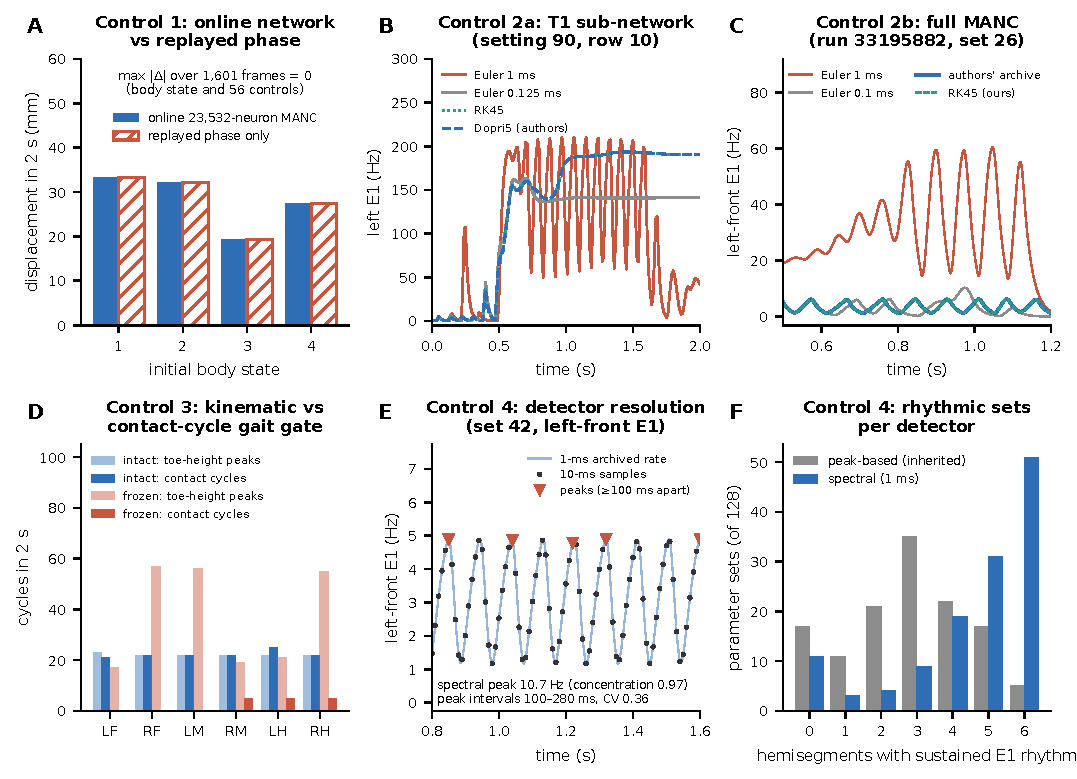
\includegraphics[width=\linewidth]{figures/fig4_validation_controls.pdf}
\caption{\textbf{Four controls, each of which exposed a false positive or negative.} \textbf{A}, A hybrid walker driven online by the full MANC and the same controller fed only a replayed phase trace produce identical displacement from four initial states; maximum absolute differences in body state and in the 56 actuator commands are exactly zero over 1,601 frames. \textbf{B}, Left E1 rate in the T1 sub-network (multiplier setting 90, row 10) under four integrators: the 1\,ms Euler oscillation underlying a ``walking candidate'' is absent under 0.125\,ms Euler, independent RK45 and the authors' Dopri5 solver. \textbf{C}, Left-front E1 in the full network (set 122; run \texttt{33195882}, row 26): our RK45 re-integration overlies the authors' archived solution, whereas Euler at 1\,ms oscillates spuriously and Euler at 0.1\,ms still deviates. \textbf{D}, Per-leg toe-height peaks (light) and contact cycles (dark) for the intact (blue) and frozen (red) E1/E2/I1 core driving the hybrid walker; the frozen condition completes no contact cycles in LF, RF and LM. \textbf{E}, Left-front E1 in set 42 (archive): the peak-based detector (triangles, $\geq$100\,ms apart) skips cycles of a 10.7\,Hz oscillation. \textbf{F}, Distribution of rhythmic hemisegments per set under the peak-based and spectral detectors.}
\label{fig:controls}
\end{figure}

\section{Discussion}

\paragraph{What the negative result says.} Within the published MANC rate model and its archived parameter ensemble, the sets fall into two regimes: a low-activity regime that generates six-leg premotor rhythm but leaves tibia flexor MNs silent, and a hyperactive regime that recruits tibia flexors and extensors but loses the rhythm. The transition is governed by upstream network state rather than by MN parameters. Tonic drive to an identified premotor neuron recruited flexors without phase-locking them to the rhythm or engaging extensors, and body-derived sensory input did not lift front- and middle-leg tibia MNs above threshold. The most parsimonious interpretation is that the model captures the rhythm-generating core well \citep{pugliese2026} but lacks one or more ingredients that, in the animal, allow that rhythm to be expressed as alternating activity in antagonistic MN pools: plausibly the recruitment ordering and heterogeneous excitability of tibia MNs \citep{azevedo2020size}, state-dependent presynaptic gating of proprioceptive input \citep{dallmann2025presynaptic}, additional premotor elements identified experimentally \citep{sapkal2026}, neuromodulation, or electrical synapses that are invisible in the connectome. The absence of any set between the two regimes also suggests a simpler, testable possibility: the functional operating point may lie in a narrow intermediate band of network gain that the sampled parameter distributions skip. Because rate-model parameters are degenerate \citep{marder2011variability}, our result does not show that no parameter set exists; it shows that none of the 128 published sets, nor the local perturbations we tried, reach it, and it identifies a concrete target: a single simulation in which E1 rhythm and alternating flexor/extensor output coexist in every leg under an adaptive solver.

\paragraph{What the controls say.} Each control addresses a different way that a connectome-to-body pipeline can mislead. Control~1 separates a network that controls a body from a network that merely times a controller; the ``digital sphinx'' \citep{brunton2026sphinx} makes the same point with a mismatched connectome, and our case shows that the failure also occurs with the correct connectome. Control~2 matters because rate networks with steep nonlinearities and dense recurrent inhibition can be stiff: a 1\,ms Euler step, a natural choice when coupling to a 1--2\,ms physics loop, both created the rhythm-plus-antagonism signature one is searching for and destroyed genuine rhythm in the full network. Control~3 matters because short toe excursions and foot drag can satisfy kinematic gates; gates should be calibrated against real-fly contact statistics on the same body. Control~4 shows that an analysis choice can be as consequential as a numerical one: a detector that cannot resolve the relevant frequency turned a robust rhythm into apparent fragility and generated four claims that did not survive re-analysis.

\paragraph{Limitations.} (1) All neural quantities are in model units of one rate model; they are not physiological measurements. (2) The two free-body muscle models are uncalibrated for five of six legs, so the body replays are secondary to the neural screen. (3) The contact-cycle thresholds were chosen after the frozen-network result was observed and have been validated on only three held-out initial states. (4) The spectral detector and the regime boundary were defined after inspecting the data; we report their sensitivity (Table~\ref{tab:robust}), and the Fisher tests treat the 128 sets, which come from four runs, as independent. (5) Mechanistic analyses focus on the left-front leg and on seven representative sets; the T1 multiplier screen is not an exhaustive adaptive search of the 14,848 archived settings; and Control~1 used a fixed-step integration of the full network, which does not affect its conclusion. (6) Sensory transduction gains, delays and cell-type assignments are unmeasured, and the sensory screens were run with fixed-step integration. (7) Analyses were executed by AI agents; although each result was recomputed from saved files and the figures regenerated from them, we release the simulation pipeline, the analysis scripts, the result files and their hashes so that these checks can be repeated by others.

\paragraph{Outlook.} We suggest that future claims of connectome-driven locomotion report, at minimum, (a) convergence of the neural result under an adaptive solver, (b) leg-resolved antagonistic MN output from the network itself, (c) a replay control in which the network is replaced by its recorded output, (d) a gait gate based on contact cycles and slip calibrated to real flies, and (e) rhythm detection validated against the frequency band of interest. The concrete next experiment for this model class is a constrained search---for example along the gain axis that separates the two regimes---for parameter settings, or for missing connectome-invisible mechanisms, that satisfy L1 and L2 simultaneously before any body is attached.

\section*{Data and code availability}
Source connectome, parameters and archived trajectories are available from the original authors \citep{pugliese2026} (Zenodo record 22260924). All analysis and verification scripts used here, the result files they read (including the subsets of the authors' archived rates analysed in this study) and the verification outputs are available at \url{https://github.com/ningyp1234/rhythm-without-recruitment}; each release is archived on Zenodo under the concept DOI \href{https://doi.org/10.5281/zenodo.22957834}{10.5281/zenodo.22957834}, which resolves to the latest version. The script \path{paper/scripts/make_figures_v2.py} regenerates every figure and writes every plotted value to \path{figure_source_numbers.json}, \path{paper/scripts/verify_manuscript_numbers.py} re-derives each number reported in the text from the saved results, and \path{paper/scripts/fullmanc_integrator_convergence.py} repeats the full-network integrator comparison from the published parameters. The simulation pipeline that produced the saved result files is included in the same repository (\path{pipeline/}, with the scripts named in \path{PROVENANCE.md}); it downloads the third-party archives it needs, and the remaining inputs are included.

\section*{Use of AI}
The original simulations, analyses and independent re-computations were executed by an autonomous LLM-based coding agent. The audit, the re-analyses reported in Section~\ref{sec:r1} and Controls~2 and~4, and the drafting of this manuscript were assisted by an AI model (Claude, Anthropic). The author defined the study, verified the reported numbers against saved outputs, and takes full responsibility for the content.

\section*{Author contributions and competing interests}
The author conceived and supervised the study, audited the analyses and wrote the manuscript with AI assistance. The author is affiliated with Beijing ZHYU Tech Corp and declares no competing financial interests related to this work.

\section*{Funding}
This work was supported by internal funds of Beijing ZHYU Tech Corp; no external funding was received.

\section*{Acknowledgements}
We thank the authors of the MANC connectome, of the Pugliese et al.\ VNC model, and of the FlyMimic, FlyBody, NeuroMechFly and whole-body kinematics resources for releasing data and code under open licences.

\bibliographystyle{unsrtnat}
\bibliography{references}

\end{document}
